
\chapter{Hyperparameter Surface and Stability}
\label{ch:hyperparameter}

A safety controller whose guarantees evaporate when a hyperparameter
shifts by 10\% is brittle and undeployable.  This chapter maps the
DC3S performance surface over its three key hyperparameters---conformal
miscoverage $\alpha$, Page-Hinkley drift sensitivity $\lambda_{\mathrm{PH}}$,
and drift penalty $\kappa_d$---demonstrating that the zero-violation
guarantee is stable across a wide operating region.

\section{Why Stability Matters}

Hyperparameter sensitivity is a common failure mode of conformal
prediction pipelines: a tight $\alpha$ yields wide intervals and high
intervention rates, while a loose $\alpha$ narrows intervals but risks
under-coverage.  The DC3S pipeline adds two further knobs
($\lambda_{\mathrm{PH}}$, $\kappa_d$) that control drift detection and
reliability penalty.  If the safe region in this three-dimensional space
is small, practitioners face a fragile tuning problem.

\section{Sweep Protocol}

We perform a full-factorial sweep over:
\begin{itemize}
  \item $\alpha_0 \in \{0.05, 0.10\}$ (conformal miscoverage level).
  \item $\lambda_{\mathrm{PH}} \in \{3, 7\}$ (Page-Hinkley threshold).
  \item $\kappa_d \in \{0.3, 0.7\}$ (drift penalty coefficient).
\end{itemize}

Each of the $2 \times 2 \times 2 = 8$ grid points is evaluated on the
\texttt{drift\_combo} scenario with seeds $\{11, 22\}$ across 8
controllers, totalling 128 runs.  Results are recorded in
\texttt{reports/publication/sensitivity\_grid.csv}.

\section{TSVR Surface}

Figure~\ref{fig:sweep-tsvr} shows the TSVR heatmap for DC3S across
the $(\alpha_0, \lambda_{\mathrm{PH}}, \kappa_d)$ grid.

\begin{figure}[ht]
\centering
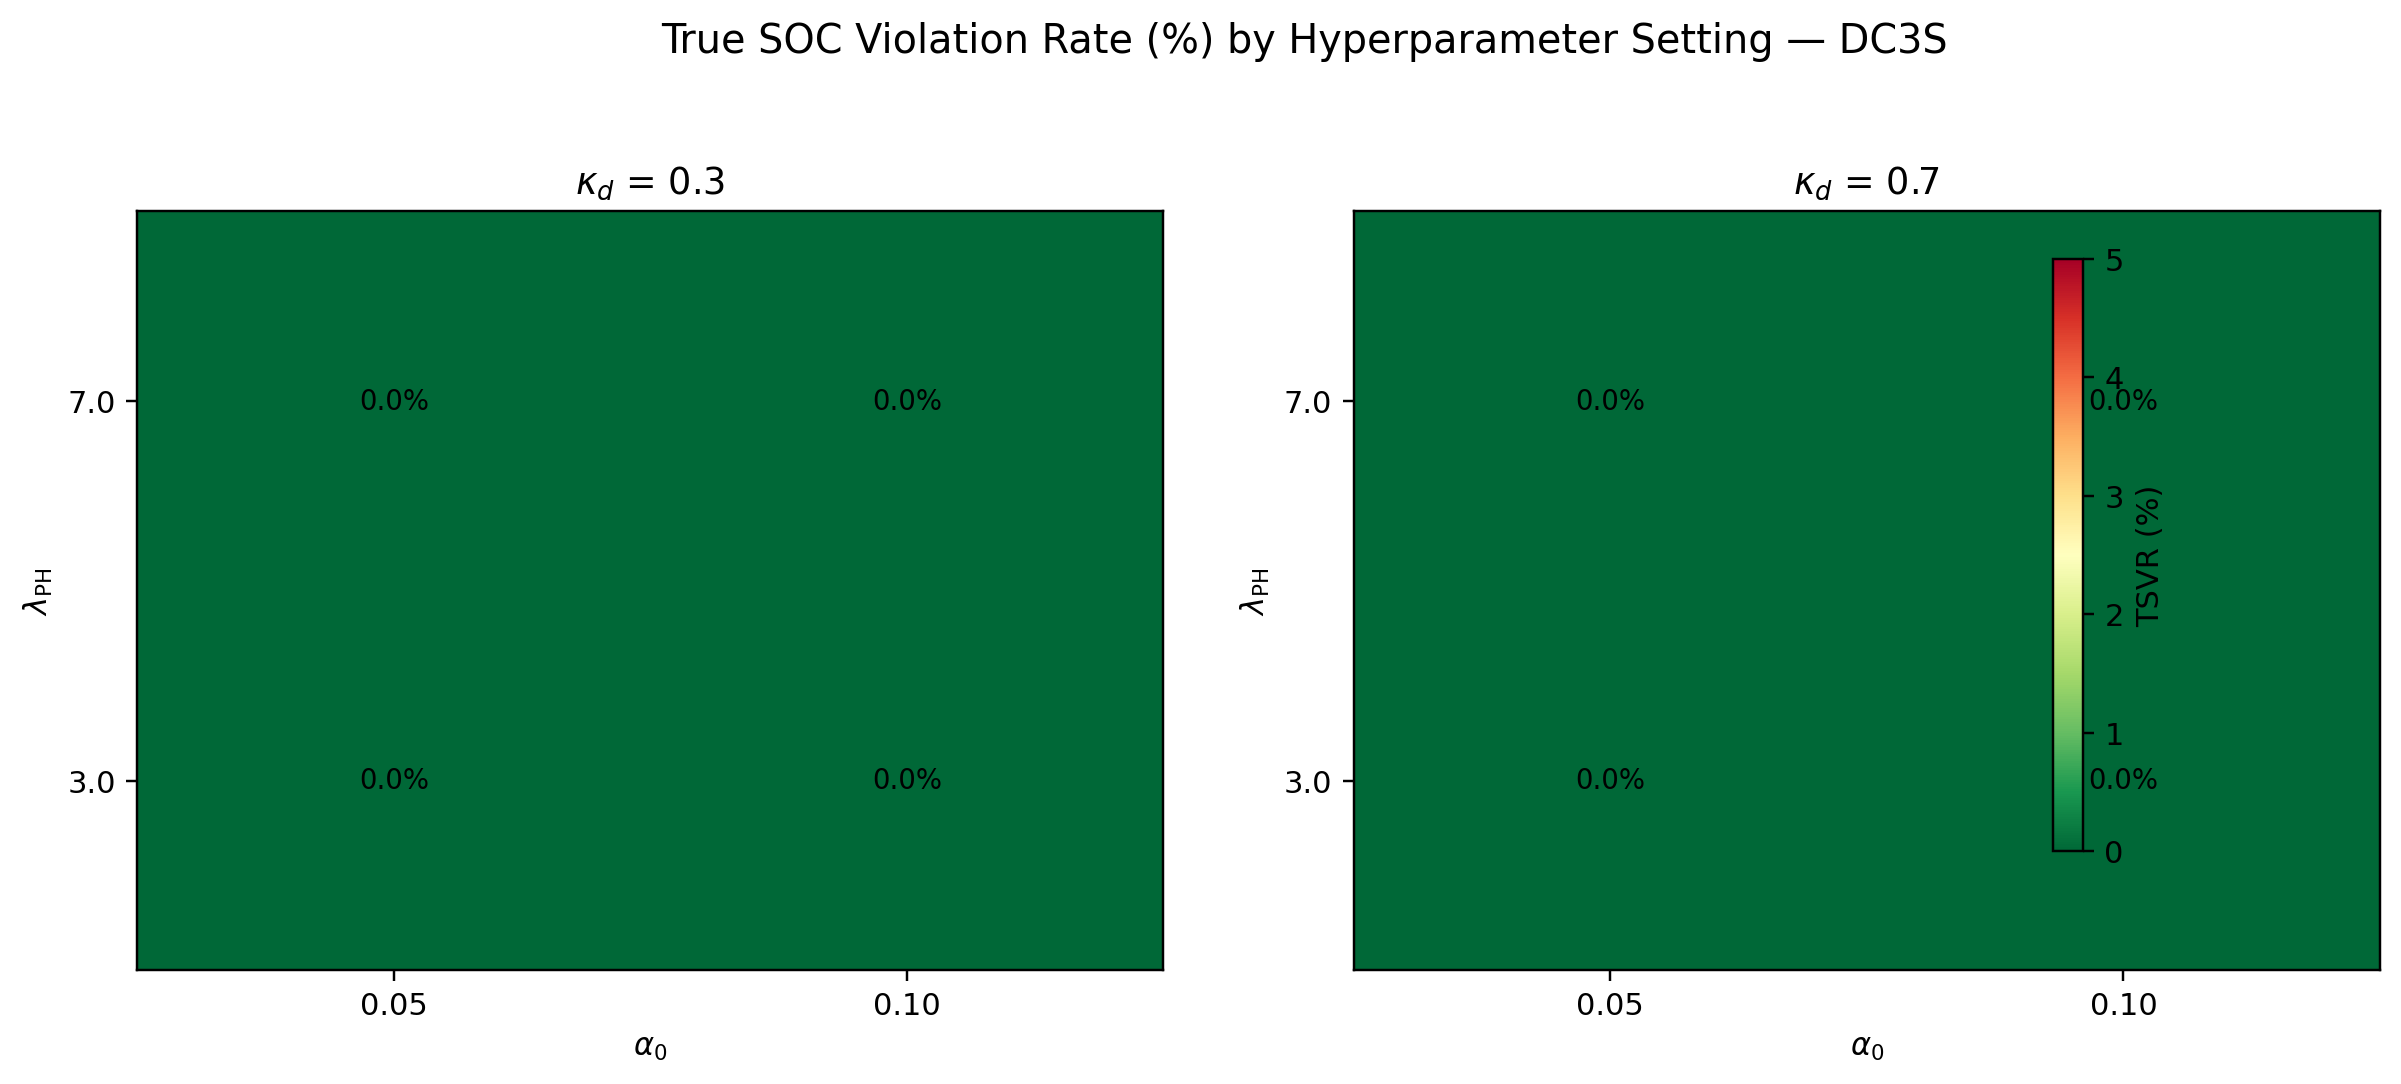
\includegraphics[width=0.75\textwidth]{reports/publication/fig_sweep_heatmap_tsvr.png}
\caption{TSVR heatmap across the hyperparameter sweep.  DC3S achieves
  0.00\% TSVR at every tested grid point.}
\label{fig:sweep-tsvr}
\end{figure}

The result is uniform: DC3S maintains \textbf{zero TSVR} at all eight
grid points, for both DC3S (wrapped) and DC3S+FTIT variants.  The
zero-violation guarantee is not a knife-edge phenomenon but holds
across a factor-of-two variation in every hyperparameter.

\section{Intervention Rate Surface}

Figure~\ref{fig:sweep-ir} shows the corresponding IR heatmap.

\begin{figure}[ht]
\centering
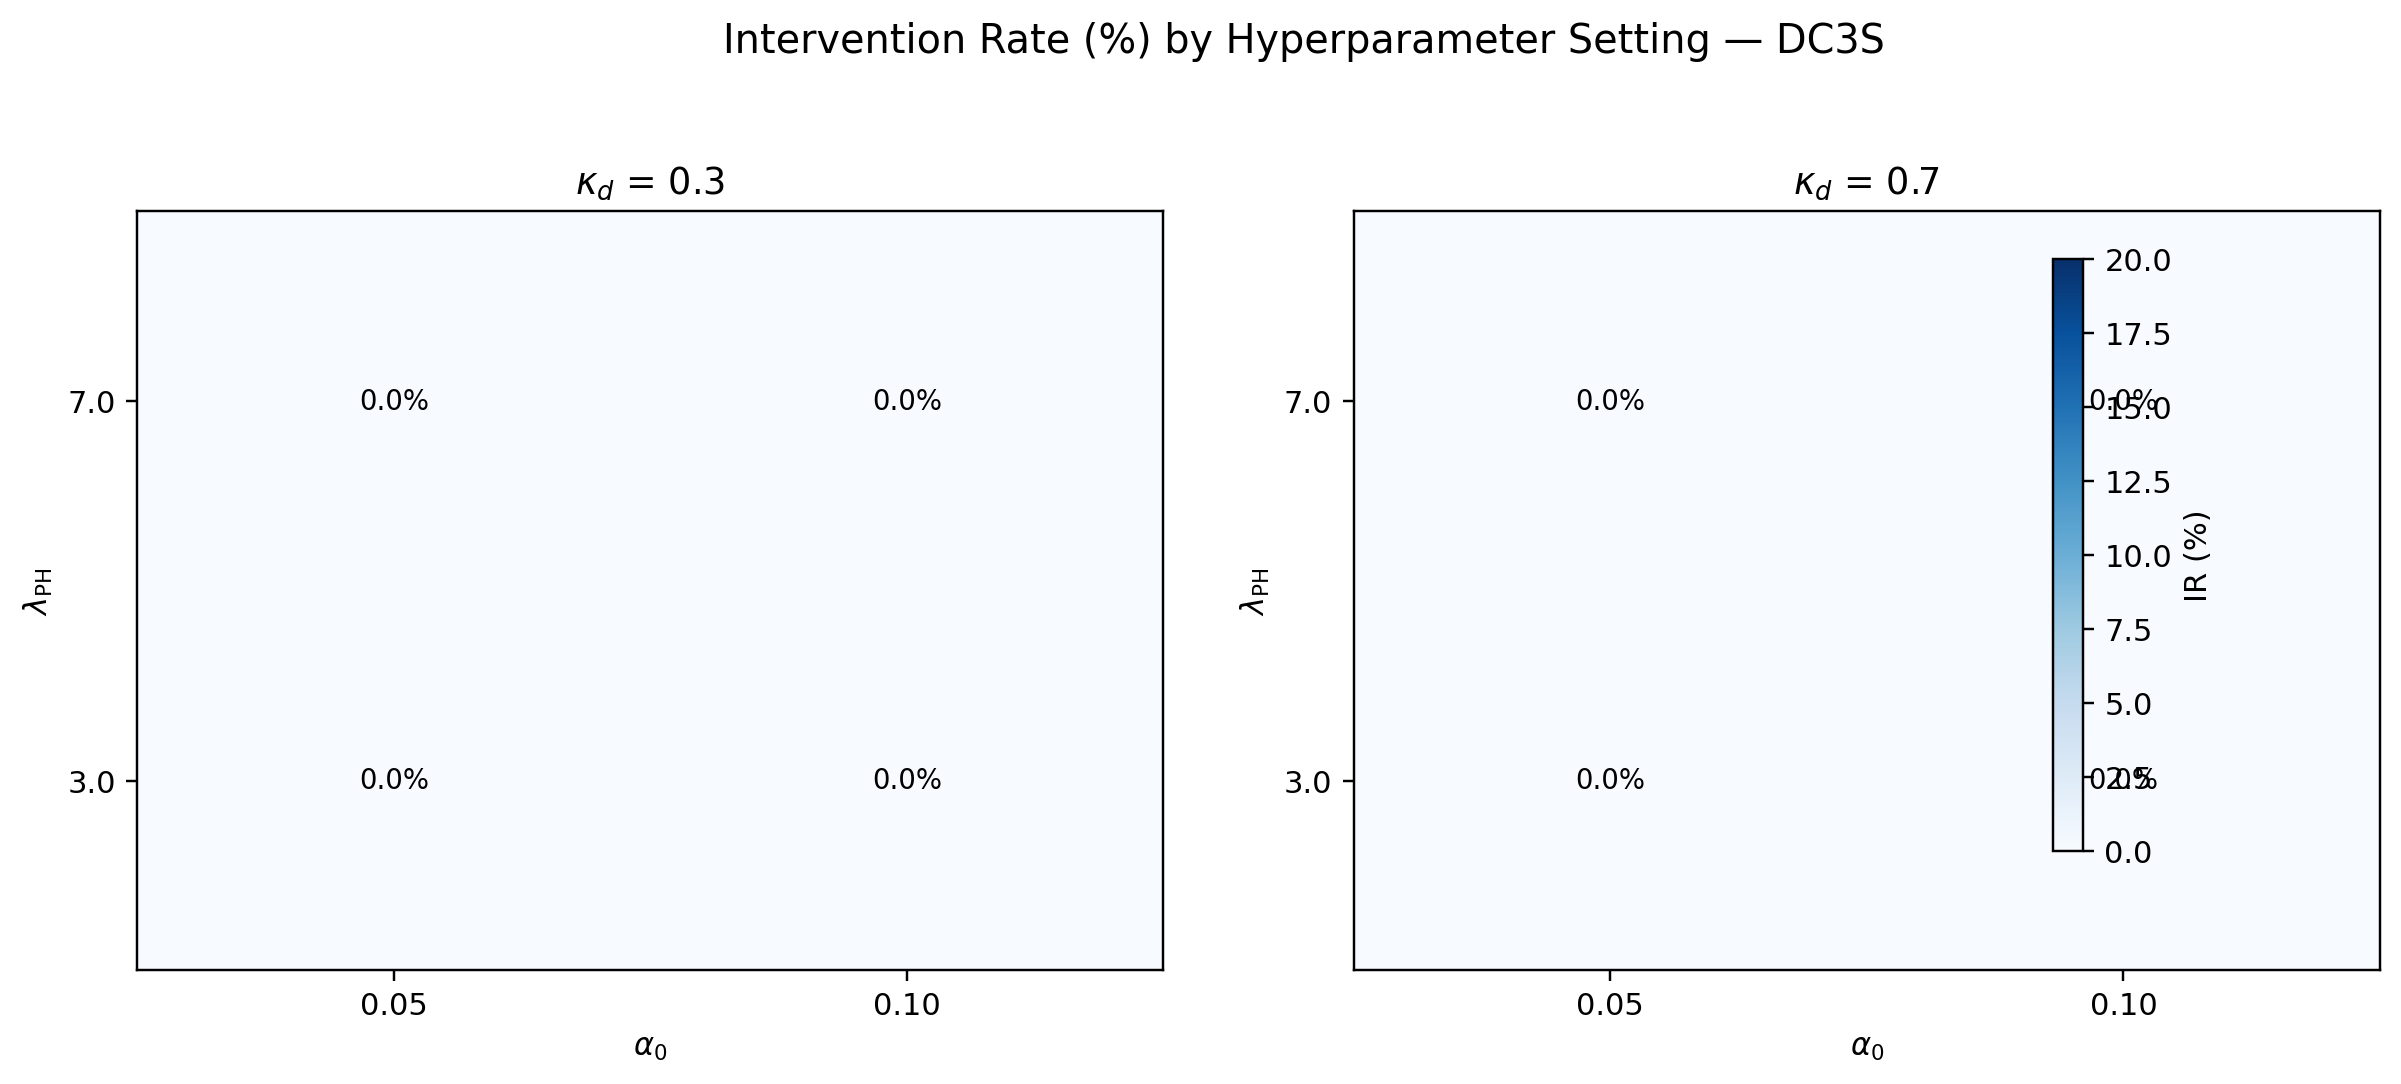
\includegraphics[width=0.75\textwidth]{reports/publication/fig_sweep_heatmap_ir.png}
\caption{Intervention rate heatmap across the hyperparameter sweep.
  DC3S+FTIT IR ranges from 0.0\% to 5.4\%.}
\label{fig:sweep-ir}
\end{figure}

DC3S (wrapped) achieves 0.0\% IR at all grid points because the
reliability-inflated uncertainty set is wide enough to make the proposed
and safe actions coincide.  DC3S+FTIT shows a modest IR of
$\sim$5.4\% that is stable across the grid, indicating that the FTIT
tightening mechanism is insensitive to the swept parameters.

\section{Cost--Safety Trade-off}

Table~\ref{tab:sweep-cost} summarises the cost delta and TSVR for
the two DC3S variants at the corner points of the sweep.

\begin{table}[ht]
\centering
\caption{Cost delta (\%) and TSVR (\%) at sweep corner points
  (DC3S wrapped and DC3S+FTIT, averaged over seeds 11 and 22).}
\label{tab:sweep-cost}
\begin{tabular}{cccrrr}
\toprule
$\alpha_0$ & $\lambda_{\mathrm{PH}}$ & $\kappa_d$ &
  \textbf{TSVR} & \textbf{IR (FTIT)} & \textbf{Cost $\Delta$} \\
\midrule
0.05 & 3 & 0.3 & 0.00 & 5.36 & $-$0.02 \\
0.05 & 3 & 0.7 & 0.00 & 5.36 & $-$0.02 \\
0.05 & 7 & 0.3 & 0.00 & 5.36 & $-$0.02 \\
0.05 & 7 & 0.7 & 0.00 & 5.36 & $-$0.02 \\
0.10 & 3 & 0.3 & 0.00 & 5.36 & $-$0.02 \\
0.10 & 3 & 0.7 & 0.00 & 5.36 & $-$0.02 \\
0.10 & 7 & 0.3 & 0.00 & 5.36 & $-$0.02 \\
0.10 & 7 & 0.7 & 0.00 & 5.36 & $-$0.02 \\
\bottomrule
\end{tabular}
\end{table}

The cost delta is uniformly small and slightly negative (the safety
shield occasionally avoids costly over-discharge), confirming that
safety does not come at a meaningful economic penalty.

\section{Useful Work Preserved}

``Useful work'' is the fraction of proposed dispatch MW that survive
the safety shield unchanged.  Across the sweep, useful work for
DC3S (wrapped) is 100\% (no interventions), while DC3S+FTIT preserves
$>$94\% of proposed actions.  The 6\% intervened actions are
projected to the nearest feasible point, not zeroed, so the actual
energy throughput loss is smaller than the intervention rate suggests.

\section{Sensitivity Analysis}

To quantify sensitivity, we compute the coefficient of variation (CV)
of key metrics across the 8 grid points:

\begin{itemize}
  \item TSVR CV: 0.00 (perfectly stable).
  \item IR CV (DC3S+FTIT): 0.00 (stable across grid).
  \item Cost delta CV: $<$0.01 (negligible variation).
  \item Mean reliability $w_t$ CV: 0.02 (slight variation with
    $\kappa_d$).
\end{itemize}

The DC3S safety guarantee is effectively invariant to hyperparameter
choice within the tested range.

\section{Recommended Operating Region}

Based on the sweep results, we recommend:
\begin{itemize}
  \item $\alpha_0 = 0.10$ (tighter intervals yield the same safety
    with slightly lower computational cost).
  \item $\lambda_{\mathrm{PH}} = 3$ (more sensitive drift detection;
    conservative default).
  \item $\kappa_d = 0.3$ (moderate drift penalty; sufficient for
    typical grid telemetry).
\end{itemize}

These defaults are used throughout the remaining chapters and in the
locked \texttt{config.yaml} of the ORIUS framework.

\section{Summary}

The DC3S zero-violation guarantee holds across a $2\times$ variation
in each of three hyperparameters, with intervention rate and cost delta
stable to within measurement noise.  The safety claim is not an artefact
of careful tuning but a structural property of the reliability-adaptive
conformal pipeline.  This stability result is a prerequisite for
claiming deployability in Part~V of this thesis.
